\documentclass[12pt]{article}
\usepackage{amsmath}
\usepackage{emptypage}
\usepackage{blindtext}
\usepackage{titlesec}
\usepackage{float}
\usepackage[hidelinks]{hyperref}
\usepackage{graphicx}
\usepackage[italian]{babel}
\graphicspath{ {./images/} }
\author{}
\title{
    \huge 
        \textbf{Università degli Studi di Modena e Reggio Emilia}
    \large
        \par Dipartimento di Scienze Fisiche, Informatiche e Matematiche
        \par Corso di laurea in Informatica
    \vfil
        \huge \par \textbf{Engim report service}
    \vfil
    \normalsize
    \begin{tabular}{lp{0.4\textwidth}l}
      Relatore: & & Candidato: \\
      Prof. Claudia Canali & &  Dumitru Frunza \\
      \end{tabular}
}
\date{Anno academico 2021/2022}
\linespread{1.5}



\begin{document}
\maketitle
\thispagestyle{empty}
\newpage 
\thispagestyle{empty}
\
\newpage
\pagenumbering{roman}
\addtocounter{page}{0}
\listoffigures
\newpage
\phantomsection
\tableofcontents
\addcontentsline{tesi}{Infrastruttura}{Infrastruttura}
\newpage
\pagenumbering{arabic}
\addtocounter{page}{0}

\section{Introduzione}
\section{Engim Srl}
\subsection{L'azienda}
Engim è una società che si occupa di creare soluzioni tecnologiche in ambito 
ICT, telecomunicazioni, sistemi di gestione e mobilità. Da oltre 10 anni operano 
nel mercato della tracciabilità di flotte e attività e della 
sicurezza dei lavoratori in solitario.
\\ ServizioGPS è il noleggio di tracker gps per veicoli lavoratori. 
Una prevalente parte dei clienti sono comuni che, tramite i prodotti Engim, 
tracciano il percorso delle macchine spazzaneve e spargisale.
I tracker possono essere prodotti fisici oppure un app per smartphone. A loro 
volta i prodotti fisici si dividono in fissi e mobili. Il servizio include
anche un gestionale per poter visualizzare, modificare o archiviare i propri dati.
\\ Twicetouch è noleggio di dispositivi di sicurezza individuale.
Il prodotto tutela i lavoratori in solitario mandando una segnalazione in caso di
emergenza. Esistono due tipi di rilevazione: 
\begin{itemize}
  \item caduta: l'accelerometro del dispositivo rileva un urto pericoloso
  \item assenza di movimento: il lavoratore non si è mosso per un lasso prolungato di tempo, 
  quindi si presume che possa essere incosciente
\end{itemize}
Similmente a servizioGPS è possibile noleggiare un dispositivo fisico (badge) oppure
l'app per android. In entrambi i casi è possibile impostare i numeri in caso di 
emergenza, che riceveranno una chiamata e un messagio SMS.

\subsection{Infrastruttura}
Le tecnologie usate per servizioGPS sono le seguenti:
\begin{itemize}
  \item Ruby on rails full stack
  \item Mariadb e Redis come database
  \item Python come back end di supporto
  \item Java per il prodotti app 
\end{itemize}
\begin{figure}[h]
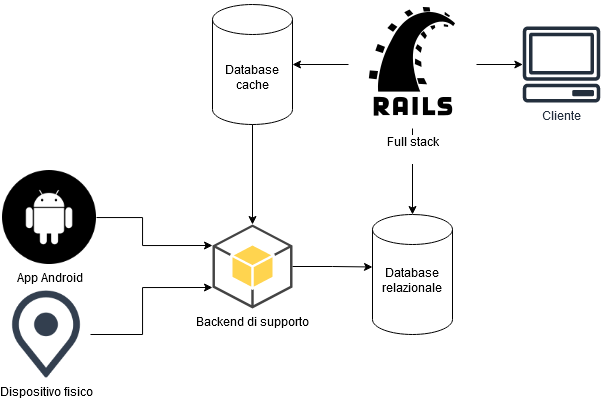
\includegraphics[scale = 0.6]{infrastructure.png}
\caption{Architettura}
\label{fig:mesh1}
\end{figure}
Ruby on Rails è usato per front-end e gran parte del backend di servizioGPS. 
Il fetcher invece si dedica esclusivamente alla elaborazione di coordinate gps,
per poter alleviare il carico di lavoro da Rails.
Allo stesso scopo il servizio si appoggia su molteplici server.
Uno di questi server è Amazon Web Services, un servizio di cloud computing 
che oltre al noleggio di un server tradizionale rende possibile 
anche un architettura a microservizi. 

\subsection{Microservizi}
Un servizio è un processo che: esegue specifiche operazioni autonomamente, 
risponde a eventi oppure rimane in attesa di una richiesta. 
Nel caso in cui queste operazioni vengano svolte continuamente, il servizio è 
estremamente vantaggioso. Non è però necessario che il servizio sia sempre in 
esecuzione se viene usato in maniera discontinua o per brevi periodi di tempo. 
I microservizi coprono questo ruolo, hanno le stesse caratteristiche di un servizio
ma eseguono solo su richiesta. 
\\ L'ambiente di esecuzione è completamente gestito da AWS, l'unica requisito per 
creare un microservizio è caricare il proprio codice. In questo caso viene 
noleggiato il tempo di calcolo invece che una macchiana fisica o virtuale.
L'ambiente viene creato al momento della richiesta, esegue il codice e cessa di 
esistere. 
Quando il microservizio non è attivo non ci sono costi.
\\ È bene tenere in mente due importanti caratteristiche dei microservizi:
\begin{itemize}
  \item L'ambiente non ha spazio di archiviazione, qualora sia necessario 
  salvare un file, bisogna caricarlo in un servizio di clound computing come S3
  \item Le tecnologie devono essere compatibili con l'infrastruttura sottostante,
  il che limita le nostre scelte
\end{itemize}
Avendo in mente queste considerazioni, un caso d'uso adatto ai microservizi 
è un servizio API che viene usato in maniera occasionale oppure per brevi periodi 
fissi.

\subsection{Sistema automatico di generazione di report}
Engim esegue una manutenzione annuale di database, che consiste nell'archiviazione
dei dati. Questi possono essere salvati dal cliente, nel caso fosse interessato 
o necessitato, sotto forma di pdf oppure xls.
\\ 
Le informazioni più importanti sono l'elenco e le specifiche di tutte le "attività". 
Un'attività contiente una serie di dati, tra cui: coordinate
gps, costi di lavoro, tempo di lavoro e altro.  
Al momento il servizio è implementato da Rails tramite una gemma di ruby. 
Il sistema attuale crea un istanza di chrome, l'istanza contiene un HTML
che si desidera convertire in pdf e infine avviene il parsing del documento.
\\ Questo ha una serie di gravi problemi:
\begin{itemize}
  \item La necessità di avviare un istanza di Chrome e il parsing di un HTML è
  estremamente costoso dal punto di vista delle risorse
  \item Il parsing di un HTML è anche estremamente costoso in termini di tempo,
  aggravato dalle lunghe query dovute alla grande mole di dati 
  \item Il  parsing tende a essere poco affidabile
\end{itemize}
La natura del nostro problema rende molto facile la scelta di un microservizio.
L'operazione è ripetitiva, ben definita e usata per brevi periodi. Altri vantaggi 
importanti sono il risparmio di risorse del server, che evita di gravare sulle 
operazioni più critiche, e la possibilità di usare il microservizio per qualsiasi 
altro prodotto Engim.


\section{Requisiti del progetto}
\subsection{Descrizione}
Il progetto è una funzione lambda su AWS, ovvero un microservizio. La funzione 
viene chiamata in maniera diretta tramite una gemma di ruby.
Questa richiede le credenziali IAM per effettuare l'accesso alla lambda e prende 
in input un json. Al suo interno abbiamo un token di autenticazione e il dominio 
di provenienza che vengono controllati dalla lambda. 
\\ I contenuti invece sono divisi in sezioni per permettere dinamicità di stampa, 
qualora uno dei blocchi fosse assente, semplicemente non verrà stampato. 
\\ Nel caso in cui la stampa sia avvenuta correttamente la funzione ritorna 200 
e il nome del file su S3. Se l'input della chiamata risulta errato, la funzione ritorna 
400 e un messaggio che descrivere l'errore. Infine se avviene un errore di connessione 
al bucket S3, la funzione ritornerà un errore 500.    
\\ Il progetto deve permettere l'implementazione di stampe diverse da quelle di servizioGPS
e di altri file di output come kml e xls. 



\subsection{Sicurezza}
L'autenticazione avviene a livello di codice, sia sul server che sul microservizio.
\\ La gemma aws-sdk-lambda permette di stabile una connessione diretta con la 
lambda. È sufficiente fornire: nome della funzione, regione, credenziali e payload. 
Le credenziali sono salvati dentro un file crittografato yaml. Nel caso in cui 
l'operazione sia andato a buon fine, ritornerà un json in risposta.
\\ AWS permette di creare variabili
d'ambiente, evitando che siano scritti in chiaro nel codice. Una di queste variabili 
è un token di autenticazione, esso viene confrontato con il token in input. 
\\ La whitelist contiene tutti i domini di Engim, questi vengono caricati in 
una lista e confrontati con il mittente. 
\\ Qualsiasi chiamata da dominio esterni oppure senza token verrà tratta come 
"400 bad request". 

\subsection{Correttezza dei dati}
Esistono 3 blocchi principali: header, body, table.
Fin tanto che almeno uno dei 3 è presente, la stampa risulta valida.
Facoltativamente è possibile includere il blocco media, che contiene 
eventuali immagini in base64. Questo blocco aiuta ad evitare la spedizione duplicata 
di immagini.
\\ Il header può contenere fino a 2 loghi, però deve necessariamente avere 
un titolo e un heading. Il heading contiene: dominio di provenienza, nome utente 
e data di oggi.
\\ Il body può contenere un numero arbitrario di blocchi. Ogni blocco è racchiuso 
in un rettangolo e a sua volta contiene una serie di titoli con i loro dati. 
È valida l'assenza di un dato, ma invalida l'assenza di un titolo. 
\\ Il table contiene una serie di titoli e una serie di righe. Non c'è limite 
al numero di righe che può contenere.
Anche in questo caso non può mancare un titolo ma un dato può essere vuoto. 
\\ Tra i tipo di dato è possibile avere un immagine, l'immagine viene spedita come 
base64, se è assente non verrà scritto nulla. 
\\ Il programma presume che i dati siano corretti, controlla solo la loro presenza.

\subsection{Problemi interni del server}
Durante l'esecuzione di una stampa vengono effettuale 3 connessioni dirette:
Rails-lambda, lambda-bucket e Rails-bucket. È possibile che una di queste 3 
fallisca, in quel caso Rails ritornerà errore 500.
\\ Nel caso in cui sia un timeout rails tenterà la connessione a lambda fin tanto 
che essa ritornerà una risposta corretta. 

\subsection{Presupposti e dipendenze}
La scelta del linguaggio è limitata da AWS, in particolare i 3 presi sotto considerazione 
sono state ruby, python e javascript. 
Le librerie di ruby prevedono il parsing di HTML quindi non risolvono i problemi 
preesistenti. 
Python offre molte librerie, ma con funzionalità parziali oppure non mantenute. 
Javascript invece ha pdfkit, una libreria che permette la creazione e manipolazione 
di un PDF senza intermezzi. 
\\ La stampa ha una forma regolare, divisa per righe e colonne. Se i dati sono 
disposti in maniera più arbitraria è necessaria un implementazione diversa. 
\\ Non è richiesto la stampa in altri formati di file, ma è necessario lasciare 
libertà di aggiunta di formati in futuro.

\subsection{Features}
La lambda ha un unica funzionalità, stampa e salvataggio della stampa.
\\ È possibile effettuare diverse stampe che hanno disposizioni simili.
\\ È possibile stampare immagini. 

\begin{figure}[H]
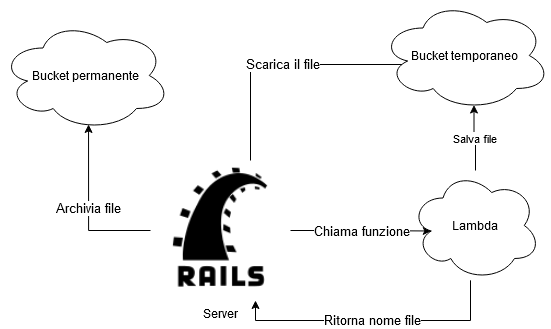
\includegraphics[scale = 0.6]{useCases.png}
\caption{Casi d'uso}
\label{fig:mesh2}
\end{figure}



\section{Implementazione}
\subsection{Flusso di lavoro}
È stato deciso di lavorare con continua integrazione. 
\\ In prima battuta creare una funzione in grado di generare un pdf e salvarlo 
su S3. Testare ogni aspetto della funzione ed effettuare il deploy su AWS. 
\\ Il secondo passaggio è integrare la funzionalità in rails, eliminando la vecchia 
integrazione. 
\\ Infine estendere questa implementazione a ogni stampa pdf sul server.

\subsection{Creazione di un file e salvataggio su S3}
La lamda è una funzione asincrona che viene eseguita ogni volta che riceve una
chiamata https. Bisogna prima di tutto creare una connessione con il bucket di s3,
una volta creata questa connessione si può salvare un file passando il filepath
oppure uno stream di data e avremo salvato il file su S3.

\subsection{Generazione di un pdf da un json}
La libreria permette scrittura sul file, disegno elementare e manipolazione di 
font, posizione e colore.
Inizialmente appariva conveniente un approccio funzionale, ma vedendo il modo 
particolare in cui viene esportato un file in nodejs e la complessità sempre 
maggiore dei documenti, è stato deciso di creare una classe: PdfDocument. 
\\
Il costruttore va a definire la grandezza del documento in base alla tabella.
Questa definisce la larghezza del documento e l'altezza viene calcolata di
conseguenza (1.41 volte più grande, come un foglio A4).
Il formato A4 è il default nel caso in cui la tabella manchi oppure la larghezza 
sia minore di un A4. 
Mantenendo queste proporzioni la visualizzazione e la stampa risultano molto 
intuitivi. 
Una volta definito il documento la classe chiama il metodo writeData. 
Questo metodo controlla la presenza dei dati e richiama altri metodi di scrittura 
se necessario.
I metodi di scrittura controllano che non manchino dati vitali e se così non fosse 
scrivono sul documento. 
È possibile richiedere il documento tramite getDocument. 
\\ 
Il file è uno stream di dati e può essere spedito su S3. 

\subsection{Test automatizzati}
La libreria aws-sdk-dev permette di simulare qualsiasi tipo di connessione aws, 
così da poter testare il collegamento con il bucket. 
Tutti gli altri test sono diversi tipi di input json e la verifica della sicurezza.

\subsection{Rails}
Rails richiede un iniziale refactoring del metodo che ritorna la stampa. Prima di 
tutto definisco che il ritorno default è pdf. Si può visualizzare oppure scaricare 
direttamente. Si stabiliscono le connessioni e poi si crea il json. Vanno caricati 
specifici dati quindi con un po' di metaprogramming diventa tutto più compatto. 
Inoltre è necessario controllare altri metodi che si appoggiano sul metodo stampa. 

\section{Applicazione e performance}
\subsection{Frontend}
Dal punto di vista del front non è cambiato nulla. Il metodi interessati sono 
activity list, report, det_report, long_report. Questi possono essere usati 
a mano da qui 
[inserire foto]
Oppure vengono chiamate una volta a settimana da questo metodo. 
[inserire codice]
\subsection{Performance}
Si può chiaramente vedere che la lambda non ha nessun problema di performance.
Essendo un super computer, anche se venissiro richiesti 10M di punti non ralentterebbe 
in maniera eccessiva il servizio. 
[grafico performance lambda]
Naturalmente quindi abbiamo due colli di bottiglia, la connessione con lambda e 
bucket e le query di rails. Le query di rails tendono a rallentare quando arriviamo 
al ordine di 100k posizioni o attività. 
[grafico query]
La connessione al bucket è molto affidabile, la connessione a lambda può richiedere 
alcuni secondi per un cold start e altri tempo aggiuntivo quando fallisce la richiesta, 
rails tenterà la funzione fin tanto che avrà un risultato corretto. 
\section{Conclusione}
\section{Appendici}
\section{Bibliografia}
\end{document}